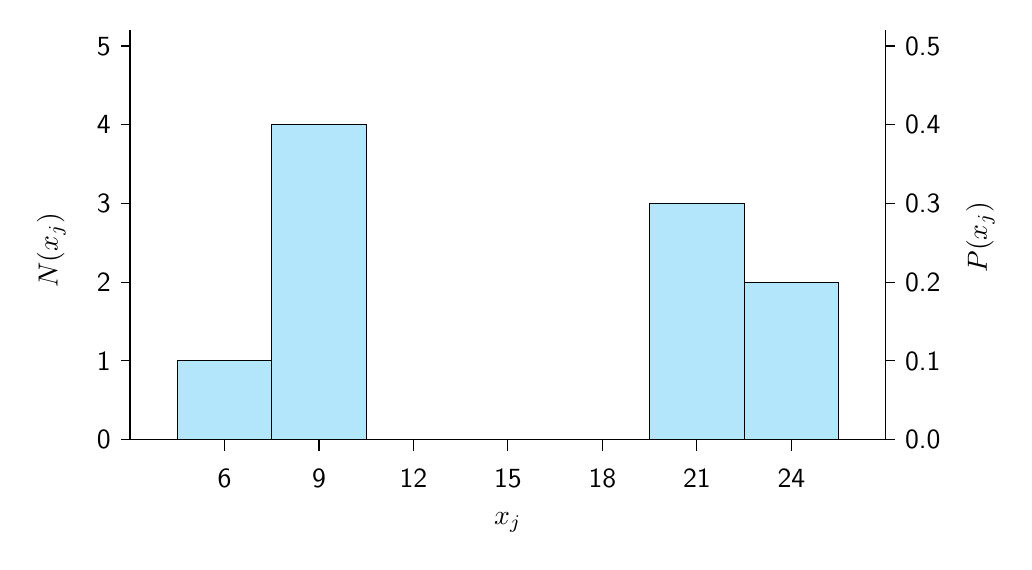
\begin{tikzpicture}[x=0.4cm, y=1cm, font=\sffamily]

% sumbu horizontal (x)
\draw (3,0) -- (27,0);

% sumbu vertikal kiri (N)
\draw (3,0) -- (3,5.2);
\foreach \y in {0,1,2,3,4,5} {
    \draw (3,\y) -- (2.7,\y) node[left] {\y};
}
\node[left=1cm, rotate=90] at (3,3) {$N(x_j)$};

% sumbu vertikal kanan (P)
\draw (27,0) -- (27,5.2);
\foreach \y/\py in {0/0.0, 1/0.1, 2/0.2, 3/0.3, 4/0.4, 5/0.5} {
    \draw (27,\y) -- (27.3,\y) node[right] {\py};
}
\node[right=1.2cm, rotate=90] at (27,2) {$P(x_j)$};

% tick sumbu x
\foreach \x in {6,9,12,15,18,21,24} {
    \draw (\x,0) -- (\x,-0.15) node[below=0.1cm] {\x};
}
\node[below=0.8cm] at (15,0) {$x_j$};

% batang histogram
\draw[fill=cyan!30] (4.5,0) rectangle (7.5,1);
\draw[fill=cyan!30] (7.5,0) rectangle (10.5,4);
\draw[fill=cyan!30] (19.5,0) rectangle (22.5,3);
\draw[fill=cyan!30] (22.5,0) rectangle (25.5,2);

\end{tikzpicture}